\documentclass[11pt,letterpaper]{article}

\pagestyle{plain}                                    

\setlength{\textwidth}{6.5in}  
\setlength{\oddsidemargin}{0in}  
\setlength{\evensidemargin}{0in} 
\setlength{\textheight}{9in}    
\setlength{\topmargin}{0in}  
\setlength{\headheight}{0in}  
\setlength{\headsep}{0in}         
\setlength{\footskip}{.35in}       

\usepackage{amsmath}
\usepackage{natbib}
\usepackage{graphicx}
\usepackage{caption}
\usepackage{authblk}
\usepackage{float}
\usepackage{lineno}
\usepackage{rotating}
\usepackage{url}
\linenumbers

\usepackage{titlesec}
\titleformat{\section}{\normalfont\fontsize{11}{11}\bfseries}{\thesection}{1em}{}
\titleformat{\subsection}{\normalfont\fontsize{11}{11}\bfseries}{\thesubsection}{1em}{}

\titlespacing\section{0pt}{11pt plus 2pt minus 2pt}{5.5pt plus 1pt minus 1pt}
\titlespacing\subsection{0pt}{11pt plus 2pt minus 2pt}{2pt plus 1pt minus 1pt}
\titlespacing\paragraph{0pt}{11pt plus 2pt minus 2pt}{2pt plus 1pt minus 1pt}

\begin{document}

\title{Wind Farm Layout Optimization with Constraints on Fatigue Caused by Partial Waking}
\date{}

\author[1]{Andrew P.J. Stanley}
\author[2]{Jennifer King}
\author[2]{Christopher Bay}
\author[1]{Andrew Ning}

\affil[1]{Department of Mechanical Engineering, Brigham Young University, Provo, UT, 84602, USA}

\affil[2]{National Renewable Energy Laboratory, National Wind Technology Center, Boulder, CO, 80303, USA}


\maketitle



\begin{abstract}
\end{abstract}

Modern wind turbines are some of the largest machines in the world. Improvements in materials technologies in recent years have allowed for taller towers, longer blades, and more power output \cite{wiser2016reducing,enevoldsen2019examining}. Because of their large size and associated large loads, as well as the cyclic loading caused by their rotational operation, fatigue is a vital consideration in wind turbine design \cite{hubler2019validation}. Turbines must be designed to operate without failure and with minimal maintenance for the duration of their lifetime, which is usually 20 years \cite{hu2016reliability,ziegler2018lifetime}. The cyclic load variations experienced by a wind turbine can be exacerbated when may turbines are built relatively close together in a wind farm. Wind turbines extract momentum from the moving air, creating a wake of slow moving wind behind them. In wind farms, turbine wakes can cause an uneven distribution of wind speeds across the swept rotor areas of downstream turbines, which intensifies the load fluctuations already present from turbulence and gravity. To make matters worse from a loads perspective, wind farms are usually optimized for maximum power production. Wind farm optimization can be used to refer to turbine layout optimization when constructing the farm, or active yaw or control to steer wakes away from downstream turbines. In each case, the objective is typically to maximize power by reducing the velocity deficits caused by wakes. This optimization often leads to partially waked turbines which can be desirable for increasing power, but devastating for the structure. In order to account for increased fatigue loading caused by partial waking in wind farms, we developed a reduced order model to quickly calculate loads which can be used to constrain turbine damage in an optimization framework. 
% We optimized wind farms in a variety of scenarios to discover the effects that additional constraints for fatigue have on optimal wind farm design.

% Lit Review
Because they are large investments and their design is driven by fatigue, many researchers have studied how different conditions affect wind turbine loading and fatigue.
% 
An early study by Thomsen and S{\o}rensen used field data and the aeroelastic code HawC to examine how different atmospheric and waking conditions affect wind turbines. They found that fatigue loading increases by 5--15\% when a turbine is operating in a wake, compared to when it is operating in the freestream \cite{thomsen1999fatigue}.
% 
Another more recent paper by Meng et al.~finds similar results to the study performed by Thomsen and S{\o}rensen. They used the large eddy simulation code SOWFA, and the finite element analysis code BECAS to find that for an open-source reference turbine, the fatigue loads increased by 16\% when the turbine operated in a wake, compared to the freestream \cite{meng2019study}.
% 
A different paper by Kim et al.~found that when the turbulence intensity was increased from around 12\% to around 20\% in a wind farm, the fatigue loads increased between 30--50\% \cite{kim2015study}. This study highlights the importance of turbulence in calculating the fatigue on a wind turbine.


In addition to characterizing fatigue loading in different conditions, several studies have been dedicating to using active control strategies to reduce fatigue loading on wind turbines. 
% 
In one of the first studies on using turbine control to reduce loads, Bossanyi showed that individual blade pitch control can be used to significantly reduce loading on the turbine structure \cite{bossanyi2003individual}.
% 
Njiri et al.~developed a control method in which the power production is slightly sacrificed to alleviate loads on the turbine structure. Near the end of a wind turbine's usual lifetime, the generator can be de-rated to extend it's lifetime. The bending moments on the blades can be reduced by more than 35\% by de-rating the generator from 100\% to 70\% \cite{njiri2019consideration}.
% 
Bernhammer et al.~performed a study with smart rotors, or rotors that use active aerodynamic devices (like flaps) to alter flow. They found that by using smart rotors the loads can be reduced by 5--15\% \cite{bernhammer2016fatigue}.

% wind farm layout optimization
The studies mentioned above use active control to reduce the loads experienced by wind turbines. There is the implicit assumption that the inflow to the wind turbine cannot be controlled. However, the inflow to a wind turbine can be somewhat controlled through layout optimization of the wind farm. With appropriate models, the loads experienced by each wind turbine in a farm can be predicted and constrained during optimization. 
Although this is a straightforward idea, current fatigue load prediction models are computationally expensive, and not suitable to be used in an optimization framework.
% 
% What We did
In this paper we present a model to quickly calculate load histories on wind turbine blades, and the associated fatigue damage. The presented model is fast enough to be used in a wind farm layout optimization, and predicts the damage trends for different waking and partial-waking conditions well compared to higher fidelity methods. 
% 
Additionally, we demonstrate using our newly presented model in a wind farm layout optimization, and show how including fatigue damage constraints change the results of the optimization.

% Brief outline
% 
% 

\section{Wind Turbine Loads Model}
\label{sec1}
In this section, we describe concepts and methods we used to estimate the loads and fatigue damage at the blade root of a wind turbine, and how the various steps and models fit together. 
% 
Before discussing the specifics of our methodology, it is important that we mention a few items. 
First, our proposed method relies on the ability to calculate the velocities and local turbulence intensities at various points throughout the wind farm. Less accurate wind farm wake models and turbulence intensity estimates will be able to predict the correct trends, but will not be as successful in predicting the actual load histories and damage values. We will discuss the models that we used and found success with. 
Second, we have validated our various models with the large eddy simulation software Simulator fOr Wind Farm Applications (SOWFA) \cite{churchfield2012nwtc}, and the aeroelastic structural analysis software OpenFAST \cite{openfast_docs}. Both of these programs are open-source, and created at the National Renewable Energy aboratory (NREL). We used the velocity data from SOWFA as the velocity input into OpenFAST to calculate the load histories on a wind turbine for various waking conditions. For the models and results shown in this paper we used the NREL 5-MW reference turbine, which is an open-source turbine design used in many research studies \cite{jonkman2009definition}.
Refer to Appendix 1 for details about our SOWFA simulations.

The rest of this section will discuss the various details of the loads and damage model that we present in this paper. 
Fatigue damage on a wind turbine is caused by cyclic loading as a turbine rotates. These load variations are caused by gravity, uneven wind speed across the rotor caused by partial waking, and turbulence. In fact, the loads on a turbine are more complicated than this, because they depend on the interactions of all of these causes.
To account for the interactions of all of these fatigue drivers, our model predicts the loads on a turbine blade at a predetermined number of azimuth angles and blade rotations. The predicted load history is then used to calculate the fatigue damage a turbine blade experiences for a given turbine layout and wind condition.
Figure \ref{flow-chart} shows a general overview the model. As each part of the model is important and has some subtleties, each will be discussed individually.
% 
\begin{figure}
    \centering
    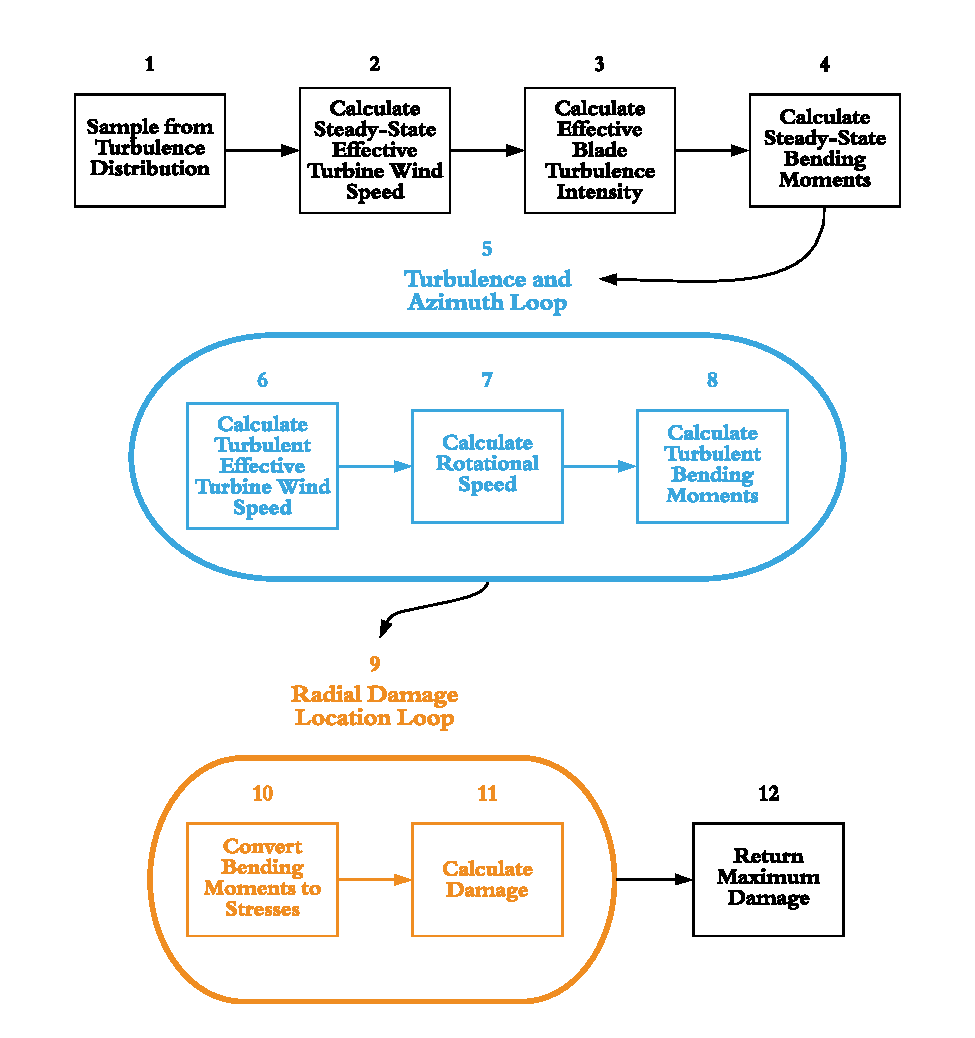
\includegraphics[]{images/fatigue-model.pdf}
    \caption{A flow chart of the damage calculation model used in this study.}
    \label{flow-chart}
\end{figure}

\subsection{Sample from the Turbulence Distribution}

The first step is to sample from a turbulence distribution. 
To account for the effect turbulence has on the loads, we added the loads caused by turbulence to the steady state loads at the desired azimuth angles, and for the selected number of rotations. Thus, the total number of turbulence samples required was the number of desired azimuth angles times the number of rotations to be modeled. 
% The results shown in this paper are for two azimuth angles, 90 and 270 degrees. These angles are when the blades are parallel to the ground on each side of the rotor, and represent the extremes of the load cycles caused by gravity and by partial waking. In addition, we modeled 100 full rotations of the rotor, meaning that we needed 200 turbulence samples.
We assumed that the velocity variations due to turbulence were Gaussian, and used Latin hypercube sampling to sample from a normal distribution with a mean of zero and a standard deviation of one.  

In addition to the values sampled, the order in which they appear is important. The model performs best when the distribution formed by taking the difference of sequential values is also approximately Gaussian. With a large enough sample, a random sample of a normal distribution will automatically meet this criterion. However, there is no guarantee for smaller samples. Thus, it is important to check that the samples and the difference of sequential values of the samples are approximately Gaussian. In this paper, we evaluated the loads at two azimuth angles for one hundred blade rotations, meaning we needed two hundred turbulence samples. The distribution we used is shown in in the left subfigure of Fig.~\ref{samples}, and the distribution formed by the difference between sequential values of the samples is shown in the right subfigure.
% 
\begin{figure}
    \centering
    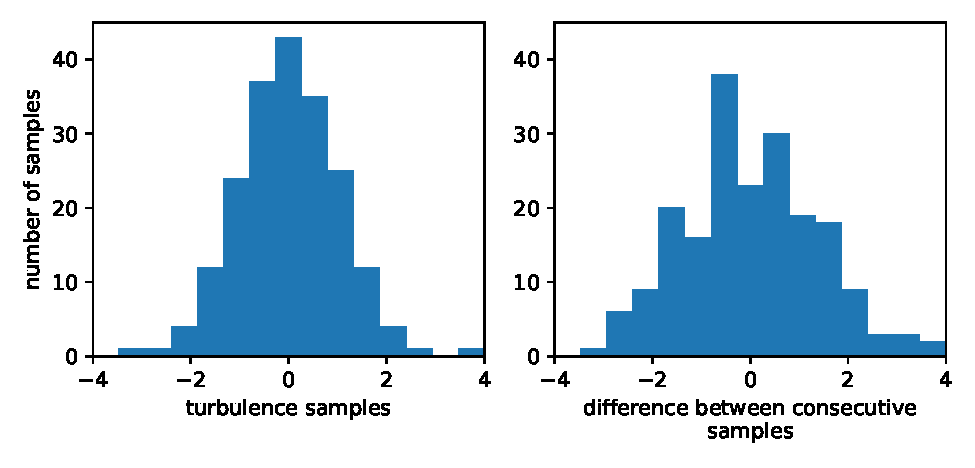
\includegraphics[]{images/turbulence_samples.pdf}
    \caption{A flow chart of the damage calculation model used in this study.}
    \label{samples}
\end{figure}




\subsection{Calculate Steady-State Effective Turbine Wind Speed}

After defining the turbulence samples, the next step is to calculate the steady-state effective turbine wind speed. This is done with an analytic wake model used to predict wind speeds in a wind farm. For this paper, we found good results with a modified Gaussian wake model presented by Bastankhah and Porté-Agel \cite{bastankhah2016experimental}.
% 
The original formulation of the model does not define the wake deficit in the near wake region, called the potential core. This creates regions behind wind turbines where the wind speed is not defined. These undefined regions in the space make optimization difficult, as the objective function is undefined is some places. To mitigate this issue, Thomas and Ning added a linear interpolation of the wake loss from the turbine up to where it is defined by the wake model, which is the version used in this paper \cite{Thomas2018}. 
The most important equation for this Gaussian wake model is shown in Eq.~\ref{wake-model}:
% 
\begin{equation}
    \label{wake-model}
    \frac{\Delta\bar{u}}{\bar{u}_{\infty}} = \Bigg(1 - \sqrt{1 - \frac{C_T \cos{\gamma}}{8\sigma_y\sigma_z/d^2}}  \Bigg) \exp{\bigg(-0.5\Big(\frac{y-\delta}{\sigma_y} \Big)^2}\bigg) \exp{\bigg(-0.5\Big(\frac{z-z_h}{\sigma_z} \Big)^2}\bigg)
\end{equation}
%
\noindent where $\Delta\bar{u}/\bar{u}_{\infty}$ is the velocity deficit in the wake; $C_T$ is the thrust coefficient; $\gamma$ is the yaw angle, which is assumed to be zero throughout this paper; $y-\delta$ and $z-z_h$ are the distances from the wake center and the point of interest in the cross-stream horizontal and vertical directions, respectively; and $\sigma_y$ and $\sigma_z$ are the standard deviations of the wake deficit, again in the cross-stream horizontal and vertical directions, respectively. These standard deviations are defined in Eqs.~\ref{sigma_y} and \ref{sigma_z}.
%
\begin{equation}
    \label{sigma_y}
    \sigma_y = k_y(x-x_0) + \frac{D\cos{\gamma}}{\sqrt{8}}
\end{equation}
%
\begin{equation}
    \label{sigma_z}
    \sigma_z = k_z(x-x_0) + \frac{D}{\sqrt{8}}
\end{equation}
%
\noindent where $D$ is the diameter of the wind turbine creating the wake, $x-x_0$ is the distance downstream from the end of the potential core to the point of interest, and $k_y$ and $k_z$ are unitless, and are functions of the freestream turbulence intensity:
%
\begin{equation}
    \label{turbulence}
    k_y,k_z = a\text{TI}+b
\end{equation}
%
In Eq.~\ref{turbulence}, $a$ and $b$ are tuning parameters, while $\text{TI}$ is the effective turbulence intensity to the upstream wind turbine. For this paper, we used the tuning parameters $a=0.4062$ and $b=0$. The length of the potential core, $x_0$ is defined in Eq.~\ref{potential_core}.
%
\begin{equation}
    \label{potential_core}
    x_0 = \frac{D \cos{\gamma} (1 + \sqrt{1-C_T})}{\sqrt{2}[\alpha^*\text{TI} + \beta^* (1-\sqrt{1-C_T})]}
\end{equation}
% 
In this equation, $\alpha^*$ and $\beta^*$ are turning parameters, for which we used the values $\alpha^*=8.059$ and $\beta^*=0$ in this paper. With the tuning parameters given, we were able to match velocity data from SOWFA very well with the analytic wake model. 
% 
Note that because the yaw angle, $\gamma$, is assumed to be zero throughout this paper, $\cos(\gamma)=1$ meaning that $\sigma_y=\sigma_z$. 

To calculate the the loads on a wind turbine in this study, we needed accurate to able to accurately predict the local turbulence intensity throughout the wind farm. Additionally, for this wake model we need the effective turbulence intensity for the inflow into a turbine. We used two different models to fit these two requirements. The model to calculate local turbulence intensity will be discussed in Section \ref{sec:TI}, while the algorithm to calculate the inflow turbulence intensity to a turbine is given in Thomas et al.~\cite{Thomas2019}.


Figure \ref{velocity_profiles} shows the velocity profiles predicted by the wake model compared to the time average velocity data from our SOWFA runs for 4, 7, and 10 diameters downstream of a wind turbine. The figure shows a horizontal sweep across the wake at hub height, at the distance downstream that is indicated. There is good agreement between the model and the SOWFA data for both high and low turbulence. With low turbulence, the wakes propagate farther, leading to larger velocity deficits downstream of the turbine. With higher turbulence, the wakes dissipate more quickly leading to smaller velocity deficits. 
% 
\begin{figure}
    \centering
    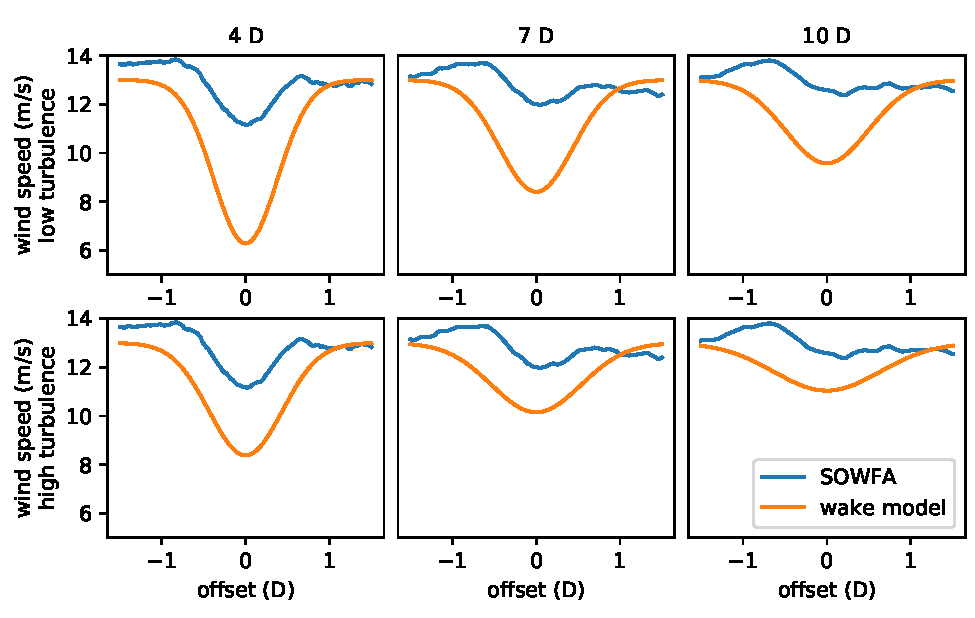
\includegraphics[]{images/velocity_profiles.pdf}
    \caption{}
    \label{velocity_profiles}
\end{figure}

If the case of combined wakes, the total wind speed was calculated with a linear combination method, represented in Eq.~\ref{combination}.
%
\begin{equation}
    \label{combination}
    \bar{u} = \bar{u}_\infty - \sum_{i=1}^\text{nTurbs} u_i \Big(\frac{\Delta\bar{u}}{\bar{u}_{\infty}}\Big)_i
\end{equation}
% 
In this equation, $\bar{u}$ is the local wind speed at a given point, $\bar{u}_\infty$ is the freestream wind speed, $\text{nTurbs}$ is the number of wind turbines upstream of the point of interest, $u_i$ is the inflow speed of an upstream turbine, and $\Big(\frac{\Delta\bar{u}}{\bar{u}_{\infty}}\Big)_i$ is the velocity deficit from an upstream turbine. This wake combination method has been shown to work well with the Gaussian wake model we used \cite{niayifar2016analytical}.

The wake model above has all been defined to calculate the wind speed at a given point. To determine the effective wind speed into a wind turbine, we took the average of the wind speed calculated at four points across the rotor, shown in Fig.~\ref{speed_samples}. We have found that sampling at these four points gives an almost identical effective wind speed as sampling with many more points across the rotor.
% 
\begin{figure}
    \centering
    \hspace*{0.7cm} 
    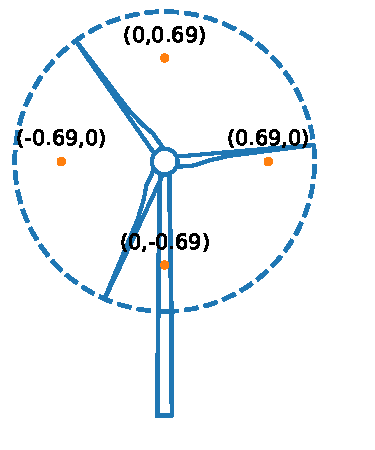
\includegraphics[]{images/rotor_samples_1.pdf}
    \caption{}
    \label{speed_samples}
\end{figure}

This section has discussed in full detail the analytic wake model we used in this paper. Remember that the fatigue model that we will present does not require this specific wake model. However, it does depend on the ability to provide accurate wind speeds for various locations throughout the wind farm. We have found success with the wake model presented in this section, however other wake models or methods to calculate the wind speed may also be used, as far as they are accurate. 

\subsection{Calculate Effective Blade Turbulence Intensity}
\label{sec:TI}

The next step in the model is to calculate the effective blade turbulence intensity at each azimuth angle, which is defined as the standard deviation of the streamwise wind speed divided by the mean. This requires the ability to accurately calculate the turbulence intensity at any given location. To accomplish this, we used a modified version of the model presented by Ishihara and Qian \cite{ishihara2018new}. This turbulence intensity model is described shown in Eq.~\ref{ti_eq}.
%
\begin{equation}
    \label{ti_eq}
    \Delta \text{TI}(x,y,z) = \frac{1}{d + e \cdot x/D + f\cdot(1+x/D)^{-2}} \cdot \Big\{k_1 \exp{-\frac{(r-D/2)^2}{2\sigma_t^2}} + k_2 \exp{-\frac{(r+D/2)^2}{2\sigma_t^2}} \Big\} - \delta(z)
\end{equation}
% 
In this equation, $\text{TI}$ is the added turbulence intensity caused by an upstream wind turbine, $x$ and $y$ are the downstream and cross-stream distances from the point of interest to the upstream turbine, $z$ is the height of the point of interest, and $D$ is the rotor diameter of the upstream turbine. The rest of the values are represented by the following equations. The values for $d$, $e$, and $f$ are given by Eqs.~\ref{d_val}, \ref{e_val}, and \ref{f_val}.
%
\begin{equation}
    \label{d_val}
    d = 2.3C_T^{-1.2}
\end{equation}
%
\begin{equation}
    \label{e_val}
    e = \text{TI}_a^{0.1}
\end{equation}
%
\begin{equation}
    \label{f_val}
    f = 0.7C_T^{-3.2} \text{TI}_a^{-0.45}
\end{equation}
In these equations, $C_T$ is the thrust coefficient of the upstream wind turbine, and $\text{TI}_a$ is the ambient turbulence intensity. The radial distance to the point of interest, $r$ , is given by Eq.~\ref{r_val},
%
\begin{equation}
    \label{r_val}
    r = \sqrt{y^2 + (z-H)^2}
\end{equation}
where $H$ is the hub height of the upstream turbine. The values for $k_1$ and $k_2$ are given in Eqs.~\ref{k1_val} and \ref{k2_val}.
%
\begin{equation}
    \label{k1_val}
    k_1 = \begin{cases} 
      \cos^2{(\pi/2 \cdot (r/D - 0.5))} & r/D \leq 0.5 \\
      1 & r/D > 0.5
   \end{cases}
\end{equation}
%
\begin{equation}
    \label{k2_val}
    k_2 = \begin{cases} 
      \cos^2{(\pi/2 \cdot (r/D + 0.5))} & r/D \leq 0.5 \\
      0 & r/D > 0.5
   \end{cases}
\end{equation}
% 
Finally, $\sigma_t$ is a representative wake width for the local turbulence intensity model, which is shown in Eq.~\ref{sigma_val}.
%
\begin{equation}
    \label{sigma_val}
    \sigma_t/D = k^* x/D + \epsilon
\end{equation}
% 
The values for $k^*$ and $\epsilon$ are given in Eqs.~\ref{k_val} and \ref{eps_val}.
%
\begin{equation}
    \label{k_val}
    k^* = 0.11 C_T^{1.07} \text{TI}_a ^ {0.20}
\end{equation}
%
\begin{equation}
    \label{eps_val}
    \epsilon = 0.23 C_T^{-0.25} \text{TI}_a^{0.17}
\end{equation}

We made some slight adjustments to this model by introducing two tuning parameters $C_1$ and $C_2$, which change Eqs.~\ref{ti_eq} and \ref{sigma_val}. The new equations are shown in Eqs.~\ref{new_ti} and \ref{new_sig}.
% 
\begin{equation}
    \label{new_ti}
    \Delta \text{TI}(x,y,z) = \frac{1}{C_1}(\frac{1}{d + e \cdot x/D + f\cdot(1+x/D)^{-2}} \cdot \Big\{k_1 \exp{-\frac{(r-D/2)^2}{2\sigma_t^2}} + k_2 \exp{-\frac{(r+D/2)^2}{2\sigma_t^2}} \Big\} - \delta(z))
\end{equation}
%
\begin{equation}
    \label{new_sig}
    \sigma_t/D = \frac{1}{C_2}(k^* x/D + \epsilon)
\end{equation}

Figure \ref{turbulence_sweep} shows the predicted turbulence intensity from the model compared to our SOWFA data. This is for a low freestream turbulence of 4.6\%. The figure shows a sweep across the turbine wake at hub height, at the indicated distance downstream. The parameters $C_1$ and $C_2$ were set to 1.2 and 2.5, respectively. Notice that there is very good agreement between the turbulence intensity predicted by the model compared to our SOWFA data.
% 
\begin{figure}
    \centering
    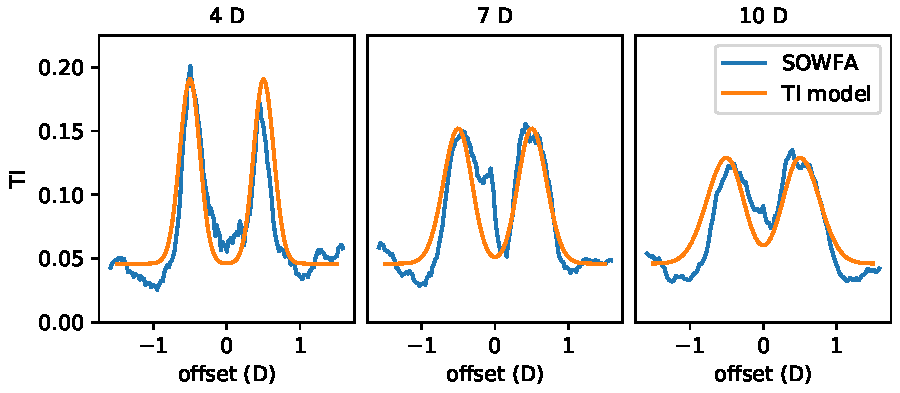
\includegraphics{images/turbulence_profiles.pdf}
    \caption{}
    \label{turbulence_sweep}
\end{figure}

With the turbulence intensity model defined, the effective turbulence intensity over the entire blade can be calculated. This is done by integrating the turbulence intensity over the length of the blade, as shown in Eq.~\ref{int_ti}.
%
\begin{equation}
    \label{int_ti}
    \text{TI}_{\text{eff}} = \frac{1}{R_{\text{tip}}}\int_0^{R_\text{tip}} \text{TI}(r)~dr
\end{equation}
%
In this equation, $\text{TI}_{\text{eff}}$ is the effective turbulence intensity over the length of the blade, $R_{\text{tip}}$ is the raidus of the blade at the tip, $\text{TI}$ is the local turbulence intensity evaluated along the length of the blade, $r$. This effective turbulence intensity for the blade is evaluated for each azimuth angle that is being considered.

\subsection{Calculate Steady-State Bending Moments}

The next step in this model is to calculate the steady state bending moments on the blade at each azimuth angle of interest. First, the loading across the blade must be calculated with the wind speeds that vary across the blade, using the same wake model described in step 2. We calculated the loads using CCBlade, a blade element momentum method for propellers and turbines \cite{Ning2020}. In addition to the wind speeds experienced across the blade, these loads are dependent on the rotor rotation speed, and the blade pitch angle. These values are determined with the turbine control scheme and the effective turbine inflow speed calculated in step 2. The rotation speeds and pitch angles as a function of inflow wind speed for the NREL 5-MW reference turbine are shown in Fig.~\ref{omegas}. 
% 
\begin{figure}
    \centering
    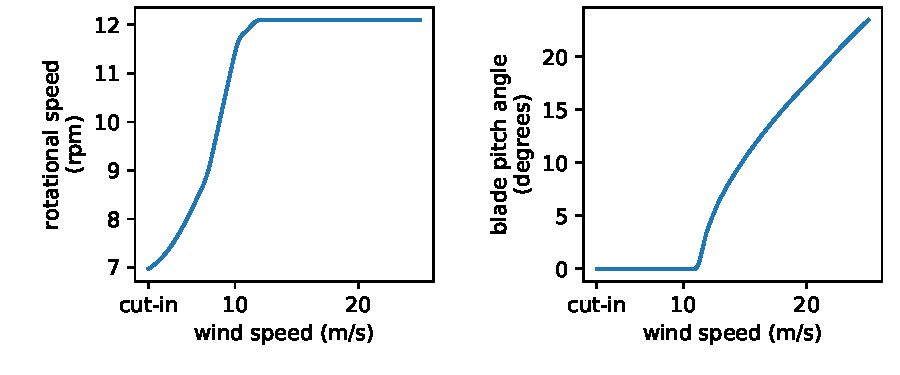
\includegraphics[]{images/omegas.pdf}
    \caption{Rotational speed versus wind speed for the NREL 5-MW reference turbine.}
    \label{omegas}
\end{figure}
% 
After calculating the loads along the blade, the moments can be determined by integrating the loads along the length of the blade, show in Eq.~\ref{int_moms}. 
%
\begin{equation}
    \label{int_moms}
    M = \int_0^{R_{\text{tip}}} Fr~dr
\end{equation}
%
In this equation, $M$ is the bending moment caused by the loading along the blade, $F$ is the loading along the blade, and $r$ is the distance along the blade.
This is done for both the edgewise and flapwise loads along the turbine blade. Because CCBlade only returns the aerodynamic loading on the blade, it is important to also add on the moment caused by gravity to the edgewise moment.

In the results for this paper, we have assumed that the fatigue critical area is at the blade root, where the bending moments are the highest. Although this may not always be the case, it is a safe assumption to demonstrate the methodology and functionality of our model.

\subsection{Turbulence and Azimuth Loop}

The three sections following this one discuss steps 6, 7, and 8. These steps occur in a loop, which creates a load history which accounts for the different azimuth angles of the blade, and the different loading that occurs each rotation from turbulence. We believe that for most cases, two azimuth angles of 90 degrees and 270 degrees are sufficient. At these angles, the gravitational loading is at the extreme values. Additionally, the load variations caused by partial waking are the largest between these two azimuth angles. In some cases with high wind shear, it may be appropriate to also include azimuth angles of 0 and 180 degrees, between which the differences in wind speed due to wind shear are the largest. However, at these angles the moments due to gravity are zero, indicating that the flapwise loads would need to be very large to introduce larger load fluctuations than would occur at azimuth angles of 90 and 270 degrees. Therefore, for most conditions just considering these two azimuth angles is sufficient. In addition to these two azimuth angles, for this paper we create our loads distribution with 100 full blade rotations. We found that this was sufficient to converge the damage values within an acceptable tolerance, while still maintaining the desired fast computational speed.

\subsection{Calculate Turbulent Effective Turbine Wind Speed}

Once in the loop, the first step is to calculate the effective turbine wind speed with turbulence. Turbulence intensity at a given point is defined in Eq.~\ref{turb_intensity}.
%
\begin{equation}
    \label{turb_intensity}
    \text{TI} = \frac{\sigma_u}{\bar{u}}
\end{equation}
% 
In this equation, $\sigma_u$ is the standard deviation of the streamwise wind speed, and $\bar{u}$ is the mean wind speed at the given point. Using this definition of turbulence intensity, we defined the instantaneous effective turbine velocity in Eq.~\ref{turbulent_inflow}.
%
\begin{equation}
    \label{turbulent_inflow}
    U_{\text{turbulent}} = U_{\text{steady}}(1 + S_i ~\text{TI})
\end{equation}
% 
In this equation, $U_{\text{turbulent}}$ is the instantaneous effective turbine inflow which accounts for turbulence, $U_{\text{steady}}$ is the steady state turbine inflow velocity calculated in step 2, and $S_i$ is the turbulence sample corresponding to the azimuth angle and rotation being calculated, which was defined in step 1. In our formulation of the model, we used the effective turbulence intensity calculated in step 3 as $\text{TI}$ in this equation (of course meaning the $\text{TI}$ corresponding to the appropriate azimuth angle). A more accurate formulation would be to calculate an effective turbulence intensity across the entire rotor, instead of using the effective blade turbulence intensity defined in Eq.~\ref{int_ti}. However, after trying both methods we found that they were graphically indistinguishable, and decided to use the blade turbulence intensity to remove a superfluous computation. 

\subsection{Calculate Rotational Speed}
This step is very simple, but can be important when calculating the damage later on. Using the control scheme of the turbine being modeled, the rotational speed of the turbine is calculated and stored based on the turbulent effective turbine wind speed calculated previously. Figure \ref{omegas} shows the rotation speed as a function of effective turbine wind speed for the reference turbine used in this study. 


\subsection{Calculate Turbulent Bending Moments}
This next critical step is to calculate the bending moment history with the instantaneous wind speeds that take turbulence into account. This could be done directly, by calling CCBlade within the turbulence and azimuth angle loop to get the blade loads, then convert them into bending moments. However, this is unnecessarily expensive. Sufficiently accurate bending moments can be calculated by simply adjusting the steady bending moment calculated in step 4 with the instantaneous turbulent wind speed. This adjustment is shown in Eq.~\ref{adjust_moms}.
% 
\begin{equation}
    \label{adjust_moms}
    M_{\text{turbulent}} = M_{\text{steady}}(1 + S_i ~\text{TI}_\text{eff})
\end{equation}
% 
As in Eq.~\ref{turbulent_inflow}, $S_i$ is the turbulence sample for the azimuth angle and cycle being computed. The moment $M_{\text{turbulent}}$ is the bending moment considering turbulence, while $M_{\text{steady}}$ is the steady bending moment that was calculated in step 4, corresponding to the appropriate azimuth angle. The turbulence intensity $\text{TI}_{\text{eff}}$ was calculated in Eq.~\ref{int_ti} of step 3, again corresponding to the appropriate azimuth angle.

Note that the moment adjustment in Eq.~\ref{adjust_moms} is made on the aerodynamic loads of both the flapwise and edgewise moments. The moments caused by gravity are unaffected by the different wind speeds. The moment histories are stored, and are used later in the model to calculated the damage.

\subsection{Radial Damage Location Loop}

After completing the turbulence and azimuth angle loop, the moment history is complete. However, the fatigue damage is dependent on the stress history, which is calculated from the moment history in the next step. The stress depends on how the flapwise and edgewise moments interact at each load cycle, and is also different depending on the location around the circumference of the blade root where the stress is calculated. Without knowing the stress history, it is impossible to know beforehand where will be the location of maximum damage. Thus, to make sure we calculate the highest fatigue value experienced by a turbine for a given loading condition, we calculated the stress history and the associated damage at several locations around the circumference of the blade root. Because exact opposite sides of the blade root experience the same stress cycle, with just the sign flipped, we only considered locations around on half of the blade root. The results shown in this paper were done with 50 stress location samples.

\subsection{Convert Bending Moments to Stresses}
Before calculating the damage, the moment history must be converted to a stress history at the location of interest. This step, along with the next, is done in a loop for each location around the circumference Finding the moments is a simple conversion, shown in Eq.~\ref{moments2stress} \cite{budynas2020shigley}.
% 
\begin{equation}
    \sigma_x = -\frac{M_z y}{I_z} + \frac{M_y z}{I_y}
    \label{moments2stress}
\end{equation}
% 
In this equation, $\sigma_x$ is the stress at the blade root, $M_y$ and $M_z$ are the moments about the $y$ and $z$ axes, respectively, $y$ and $z$ are the distances from the center of the blade root to the location of interest in the $y$ and $z$ directions, and $I_y$ and $I_z$ are the second moments of inertia about the $y$ and $z$ axes, respectively. We assume the the blade root is a hollow cylinder, for which the moment of inertia is given in Eq~\ref{moment_inertial}.
% 
\begin{equation}
    I_y = I_z = \frac{\pi}{4} (R_\text{outer}^4 - R_\text{inner}^4)
    \label{moment_inertial}
\end{equation}
% 
In this equation, $R_\text{outer}$ represents the outer radius of the blade root, and $R_\text{inner}$ represents the inner radius. For the NREL 5-MW reference turbine, these values are 1.771 meters, and 1.711 meters, respectively. Note that for these equations we are using the axes aligned with the wind farm, where the $x$ axis is in the freestream wind direction, the $y$ axis is in the cross-stream direction, and the $z$ axis is vertical. As seen in Eq.~\ref{moments2stress}, we have ignored the contributions from the shear forces in the stress calculations. After testing, we found that the contribution from shear was negligible compared to the bending moments, because of the large moment arms. 


\subsection{Calculate Damage}

From the stress history, the damage accumulated by a wind turbine throughout its lifetime is calculated for the given load conditions.
First, rainflow counting was used to determine all of the stress cycle ranges and peaks. Rainflow counting is a commonly used method to extract all of the loading cycles that occur in a noisy set of data \cite{matsuishi1968fatigue}.
A Goodman correction was then applied to account for the mean loading effects, and extract an equivalent fully reversed load:
\begin{equation}
    \sigma_{er} = \frac{\sigma_a}{1-\sigma_m/\sigma_U}
    \label{goodman}
\end{equation}
\noindent where $\sigma_{er}$ is the effective fully reversed stress amplitude, $\sigma_{a}$ is the stress amplitude for a given stress cycle, $\sigma_{m}$ is the mean stress of the stress cycle, and $\sigma_{U}$ is the material ultimate stress, which was assumed to be 70 GPa at the blade root \cite{mandell2003new}.
% @inproceedings{mandell2003new,
%   title={New fatigue data for wind turbine blade materials},
%   author={Mandell, John F and Samborsky, Daniel D and Wang, Lei and Wahl, Neil K},
%   booktitle={ASME 2003 Wind Energy Symposium},
%   pages={167--179},
%   year={2003},
%   organization={American Society of Mechanical Engineers}
% }
% 
The cycles to failure for each effective fully reversed load were then calculated as done in mLife, a wind turbine fatigue calculation code
\cite{hayman2012mlife}:
% 
\begin{equation}
    N_{\text{fail}} = \Big(\frac{\sigma_U}{\sigma_{er}*SF}\Big)^m
    \label{cycles}
\end{equation}
%
\noindent where $N_{\text{fail}}$ is the number of cycles to failure, $SF$ is a safety factor, and $m$ is the material dependent W\"{o}hler exponent. For composite turbine blades, it is typically assumed that $m=10$, which is the value used in this study \cite{Ingersoll2018}. 
Miner's rule was then used to calculate the damage accumulated by a turbine over a 25-year lifespan, shown in Eq.~\ref{miners}:
\begin{equation}
    d_i = \frac{N_{\text{cycles},i}}{N_{\text{fail},i}}
    \label{miners}
\end{equation}
\noindent where $d_i$ is the damage accumulated by the blade at the specified location around the blade circumference and $N_{\text{cycles},i}$ is the number of cycles that the blade experiences at the given loading condition. 
The number of cycles a blade would experience at a given condition over its lifetime is defined in Eq.~\ref{ncycles}:
% 
\begin{equation}
    N_{\text{cycles},i} = \frac{86400 \cdot 365.35 \cdot P_i ~ N_{\text{years}}~ N_{\text{count}}}{t_{\text{simulated}}}
    \label{ncycles}
\end{equation}
% 
where 86,400 is the number of seconds in a day, 365.25 is the number of days in a year, $P_i$ is the probability of the loading condition occurring, $N_{\text{years}}$ is the desired lifetime of the wind turbine which was assumed to be 25 years for this study, $N_{\text{count}}$ is the number of times the given loading condition happened during the simulation (this was extracted with the rainflow counting), and $t_{\text{simulated}}$ is the total time of the simulation. The equation defining $t_{\text{simulated}}$ is given in Eq.~\ref{t_sim}.
% 
\begin{equation}
    t_{\text{simulated}} = N_{\text{cycles}} \frac{2\pi}{\Omega}
    \label{t_sim}
\end{equation}
% 
In this equation, $N_{\text{cycles}}$ is the number of rotor rotations included in the simulation, which was 100 for the results shown in this paper, and $\Omega$ is the average of the rotor rotation speed, a history of which was calculated in step 7. 
                
% This process was then repeated for each turbine and for each wind direction. The total damage accumulated by each turbine (Eq.~\ref{damage}) is represented as the sum of the damage from each loading condition.
% %what do you mean by which?
% The turbine damage is a function of the flow field, which depends on the wind farm layout and wind direction:
% \begin{equation}
%     D = \sum_{i=1}^\text{nDirs}d_i
%     \label{damage}
% \end{equation}
% \noindent where D is the total damage accumulated by a turbine and nDirs is the number of wind directions considered in the analysis.


\subsection{Return Maximum Damage}

Finally, after calculating the fatigue damage at each of the locations around the blade root circumference, return the maximum damage value. 
We tested the model for a variety of loading conditions and found that, for the situations that we tested, the locations of maximum damage were all within ten degrees of each other.
Returning the maximum damage is a conservative approach, which is the equivalent of saying that the highest fatigue damage experienced around the blade root for a given load history is experienced everywhere around the blade root. 
A more exact method would be to store the damage experienced at each location separately, however our testing implies that returning the maximum damage is an appropriate simplification.




\section{Comparison of Fatigue Model to SOWFA/FAST Data}
With our new model explained in Sec.~\ref{sec1}, this section will show how it compares to the high fidelity LES and loads simulations. All of the comparisons shown in this section demonstrate the damage a turbine experiences for different amounts of partial waking. In each scenario, there is one fixed upstream turbine, while a second turbine is moved across the wake. The damage to the downstream turbine is shown for each location across the wake. Because of the computational expense required for the SOWFA and OpenFAST runs, the data points are more scarce than those for our new model. As was said earlier, these results shown are for the NREL 5-MW reference turbine. The turbulence samples for these results are shown in Fig.~\ref{samples}, and there is a safety factor of 1.15. Figures \ref{low_TI} and \ref{high_TI} show how our model compares to the high fidelity SOWFA and OpenFAST data for a lower turbulence intensity case of 4.6\%, and a higher turbulence intensity case of 8\%. In these two figures, we show the damage results for wind speeds of 10, 11, and 12 meters per second. These wind speeds are near rated speed, where the pitch angle is zero or very small, which means these wind speeds should experience the highest normal operation load fluctuations and associated fatigue damage.

Figure \ref{low_TI} shows how our model compares to the high fidelity data for the low turbulence case. The model matches the SOWFA and OpenFAST data very well, across all of the turbine spacings and wind speeds shown. Not only are the trends correct, but the magnitude of the damage prediction is remarkably close to the higher fidelity data. This is particularly impressive because the damage value is dependent on so many calculations that are required with high precision to match at this level. 
Figure \ref{high_TI} shows how our model compares to the high fidelity data for the high turbulence case. In this figure we can see that the model very well predicts the correct trends. The offset location of peak damage is correct, and the relative differences between the different wind speeds and turbine spacings are well represented. Unlike the low turbulence case however, the magnitude of the damages predicted by our model are not as accurate. We significantly underpredict the damage, especially for the highest wind speed of 12 meters per second, and for the closest turbine spacing of four rotor diameters.
% 
\begin{figure}
    \centering
    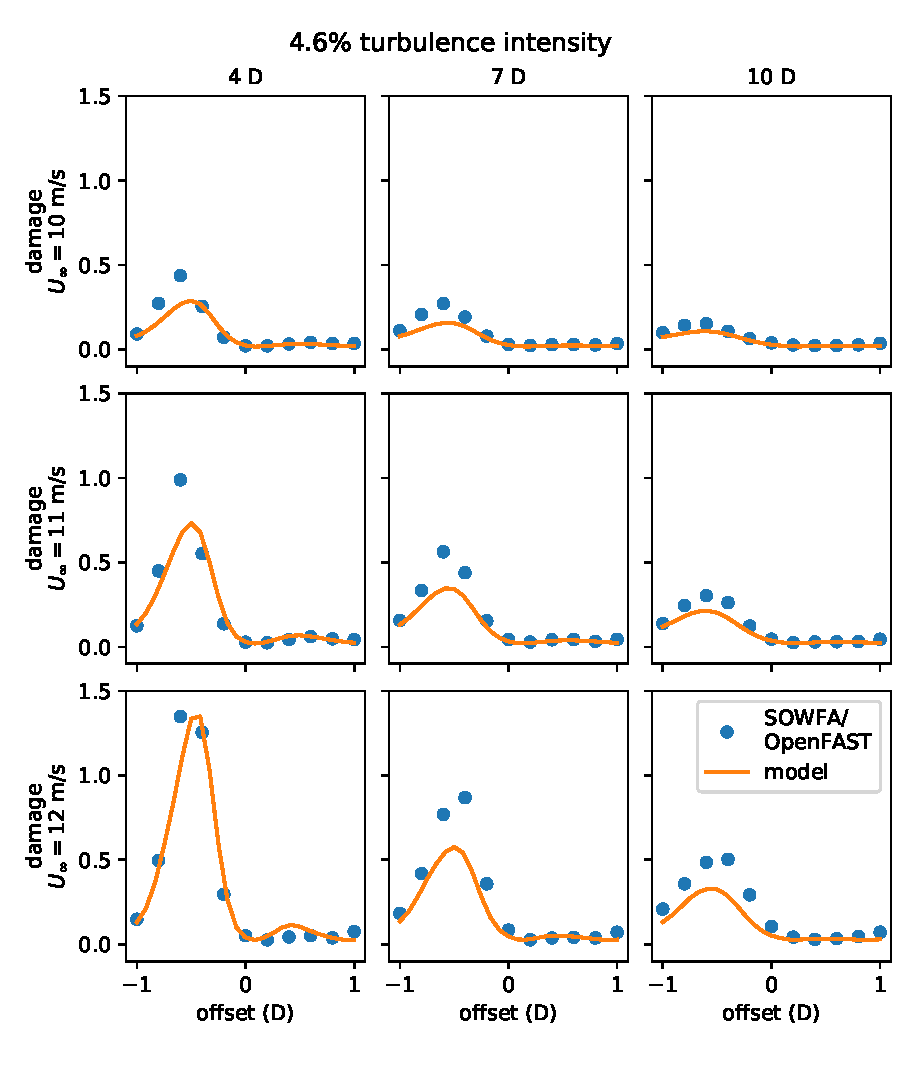
\includegraphics{images/lowTI_damage.pdf}
    \caption{}
    \label{low_TI}
\end{figure}
% 
\begin{figure}
    \centering
    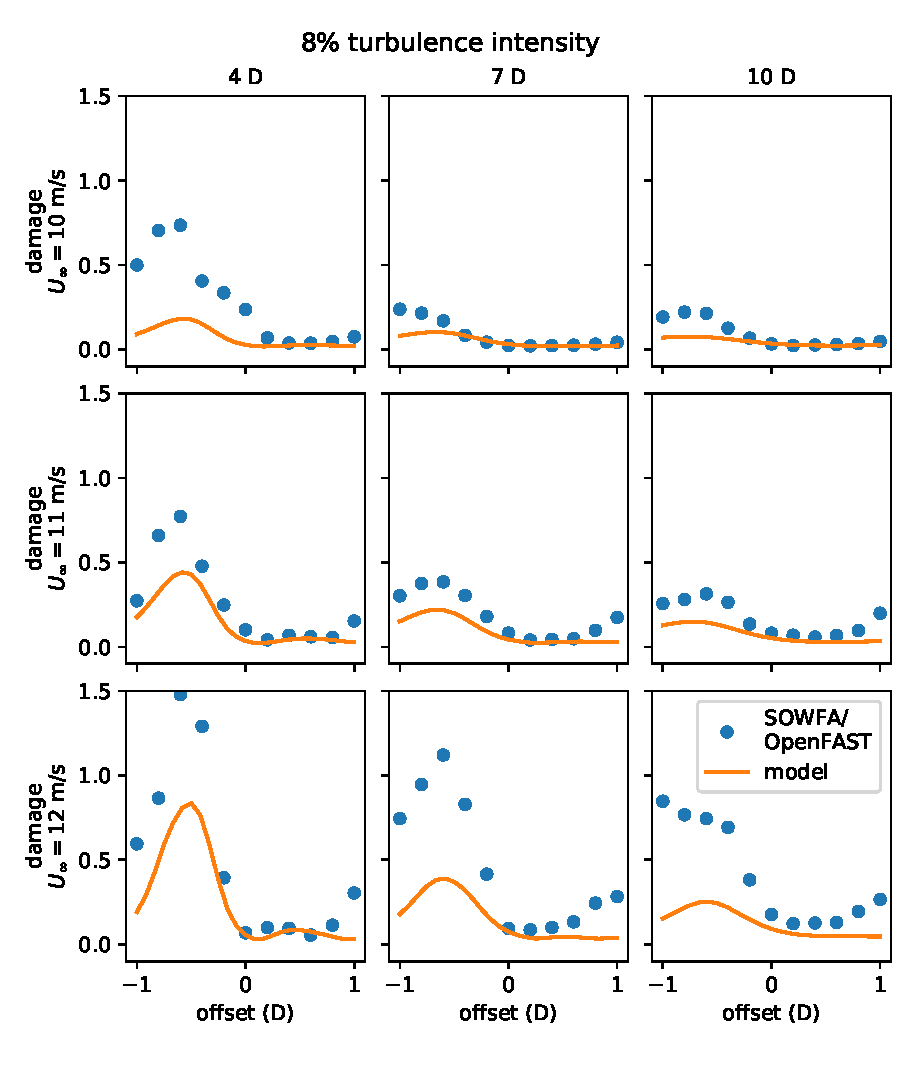
\includegraphics{images/highTI_damage.pdf}
    \caption{}
    \label{high_TI}
\end{figure}
% 

For wind speeds lower than those shown in Figs.~\ref{low_TI} and \ref{high_TI} (0--10 meters per second), our model matches the SOWFA and OpenFAST data very well. However, with the current formulation of our model we are massively underpredicting the damage at higher wind speeds. Figure \ref{thirteen} shows the damage value comparisons for the low turbulence case and a wind speed of thirteen meters per second. As can be seen in this figure, our model is predicting very little damage, while the high fidelity data is still indicating that significant damage occurs for a partially waked turbine at this wind speed. This wind speed is above the rated wind speed for the wind turbine, and is high enough that even when the downstream is waked or partially waked it is above the rated wind speed. This means that, in theory, the blades would be pitched which would dramatically decrease the loading. While this is what our model predicts in the current formulation, the SOWFA and OpenFAST data for this scenario predicts lower pitch angles than we are in the model, which is at least partially responsible for large differences in the damage predictions.
% 
\begin{figure}
    \centering
    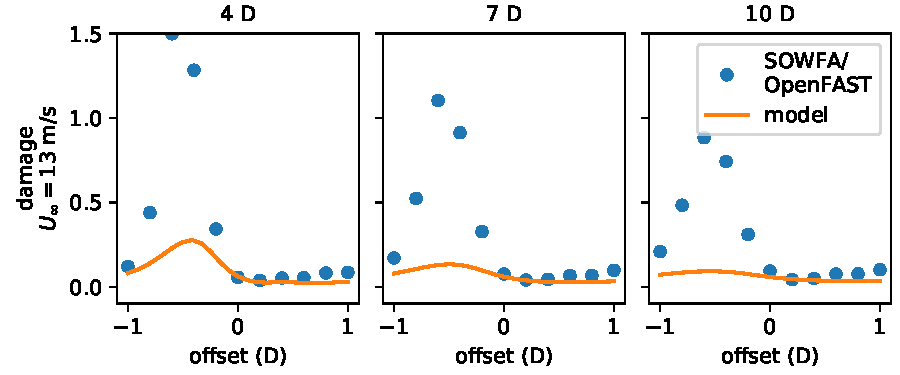
\includegraphics{images/damage_13.pdf}
    \caption{}
    \label{thirteen}
\end{figure}

One observation that is consistent across all of the results shown in Figs.~\ref{low_TI}--\ref{thirteen} is that the fatigue damage is higher when the turbine is partially waked on one side (with a negative offset in how we have presented the data), but the damage is slightly lower or at least unaffected when it is partially waked on the other side. While at first this may seem unintuitive, there is a simple explanation for this behavior caused by the interaction of the gravitational loads and the edgewise aerodynamic loads. If the blade is partially waked while rotating upwards, the aerodynamic loads on the blade will be relatively lower. This means there is a smaller force to offset the gravitational loads, and the load fluctuations will be higher than if the turbine is operating in freestream conditions. On the other hand, if the blade is partially waked while rotating downwards, the aerodynamic loads acting in the same direction as the gravitational force are relatively lower. In this configuration, the load fluctuations are smaller than in freestream operating conditions. These interactions are explained more clearly in Fig.~\ref{partial_loading}.
% 
\begin{figure}
    \centering
    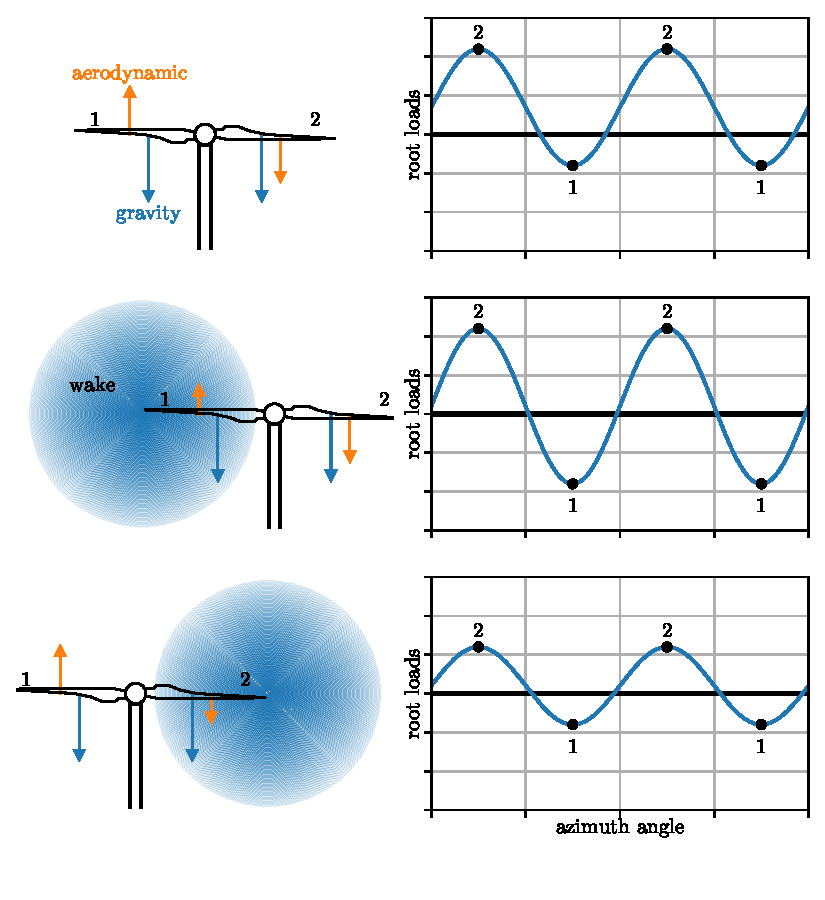
\includegraphics{images/partial_loading.pdf}
    \caption{Exaggerated edgewise load differences for different waking scenarios. Shown conditions are freestream, partially waked that increase load fluctuations, and partially waked that decrease load fluctuations. The different combinations of the gravitational force and the aerodynamic force along the blade cause different load fluctuations. Blade positions 1 and 2 are labeled on the turbine figures on the left, which correspond to the numbered points in the loading figures on the right. }
    \label{partial_loading}
\end{figure}

\section{Example Optimization}

In this section we will discuss a representative wind farm layout optimization in which we used our model to constrain the damage caused by partial waking throughout the wind farm. Before discussing the optimization and the results, we'll briefly describe the models and assumptions we've made for this optimization. This optimization considers a wind farm with 40 turbines. As with the rest of this paper, this wind farm layout optimization assumed the NREL 5-MW reference turbine design throughout the farm. This turbine has a rotor diameter of 126.4 meters, a hub height of 90 meters, a cut-in wind speed of 3 meters per second, a rated wind speed of 11.4 meters per second, and a rated power of 5 megawatts. The power curve for this turbine was assumed to be perfectly cubic, as represented in Eq.~\ref{power_curve}. 
% 
\begin{equation}
    P = \begin{cases} 
      0 &  U_\text{eff} < U_\text{cut-in} \\
      (U_\text{eff}/U_\text{rated})^3 P_\text{rated} &  U_\text{cut-in} \leq U_\text{eff} < U_\text{rated}\\
      P_\text{rated} & U_\text{eff} \geq U_\text{rated}
   \end{cases}
   \label{power_curve}
\end{equation}
% 
In this equation, $U_\text{eff}$ is the effective inflow speed to the turbine, $U_\text{cut-in}$ is the cut-in wind speed, $U_\text{rated}$ is the rated wind speed, and $P_\text{rated}$ is the rated power.
We assumed wind speeds that were all relatively low, and thus did not need to consider a cut-out wind speed.
Additionally, we assumed the turbines always faced directly into the oncoming wind, that the terrain was flat, and a safety factor of 1.25 for the fatigue calculations.

Figure \ref{windrose} shows the wind rose and wind speed distributions we used for this study. This wind probability distribution is from the Horns Rev wind farm, as is the wind speed distribution, except we increased all of the wind speeds by three meters per second so they were closer to the rated wind speed of the NREL 5-MW reference turbine. We used 24 wind direction bins (every 15 degrees), and assumed directionally averaged wind speeds. We assumed a wind shear exponent of 0.15, and a freestream turbulence intensity of 4.6\% (corresponding to Fig.~\ref{low_TI} for the damage calculations).

The objective of this optimization was to maximize the annual energy production (AEP) of the wind farm with respect to the location of each turbine. The rotor hubs were constrained to be at least two rotor diameters apart from each other. Additionally there were boundary constraints which forced the turbines to remain in a fixed wind farm boundary. The size of the boundary resulted in an average turbine spacing of about 5.2 rotor diameters. Finally, the total fatigue damage was constrained to be less than 0.2. When considering fatigue damage, the assumption is that failure occurs when the damage value reaches unity. However, with the layout optimization we are only considering the additional damage caused by waking and partial waking of the wind turbines. Other significant drivers of fatigue are extreme wind gusts and cases of extreme wind shear and veer. There phenomena are not captured with our presented model, therefore we must constrain the optimization to some value less than one. Although our chosen value of 0.2 is arbitrary, it is sufficient for this example optimization in demonstrating the capabilities of our model. If full, this optimization is represented in Eq.~\ref{optimization}.
% 
\begin{equation}
			\begin{aligned}
				& \text{maximize}
					& & \text{AEP} \\
                & \text{w.r.t.} 
                	&& x_j,~ y_j ~ (j = 1, \ldots, 40)\\
				& \text{subject to}
					& & \text{boundary constraints} \\
						&&& \text{spacing constraints} \\
						&&& \text{damage}_j < 0.2 ~ (j = 1, \ldots, \text{nTurbines})
			\end{aligned}
		\label{optimization}
		\end{equation}

In order to provide a point of reference and find a starting point for our final optimization with damage constraints, we first ran 200 optimizations of the wind farm without damage constraints and with randomly initialized design variables. We then chose the layout with the highest AEP, and used that as the starting point for our optimization with loads constraints.
\begin{figure}
    \centering
    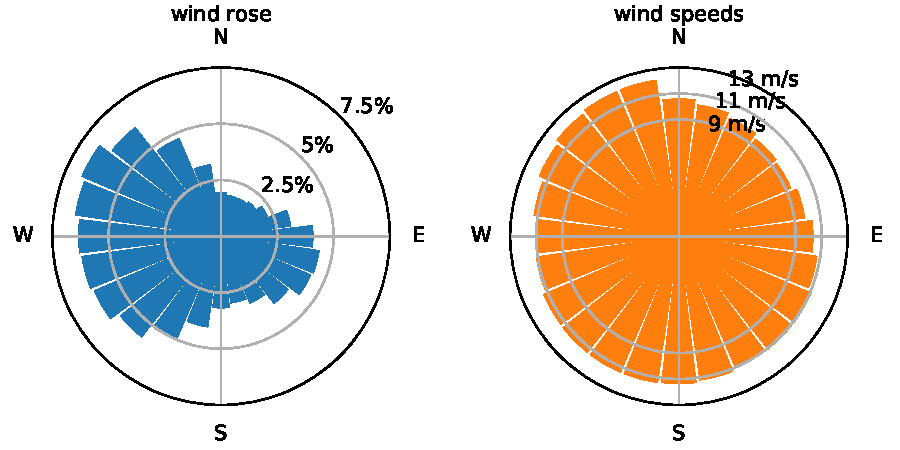
\includegraphics{images/windrose.pdf}
    \caption{}
    \label{windrose}
\end{figure}

\begin{figure}
    \centering
    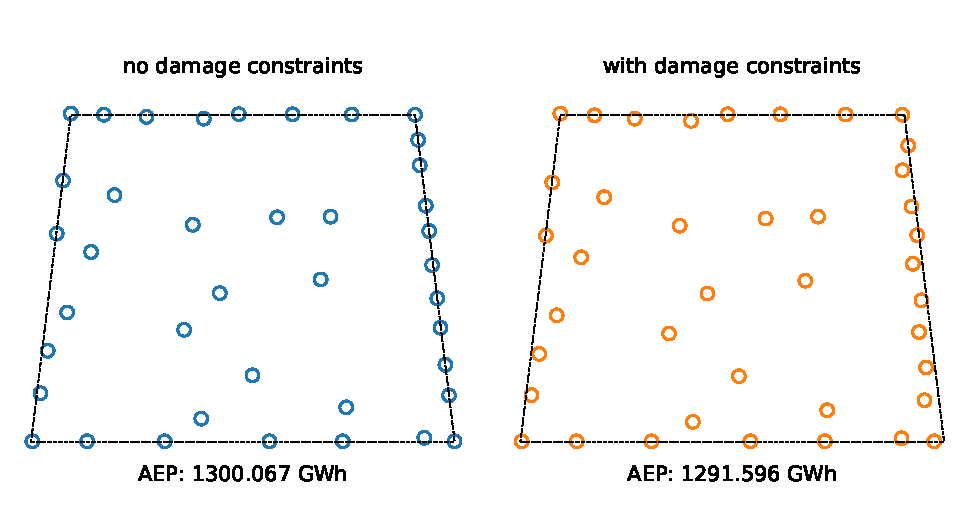
\includegraphics{images/opt_layouts.pdf}
    \caption{}
    \label{layouts}
\end{figure}

\begin{figure}
    \centering
    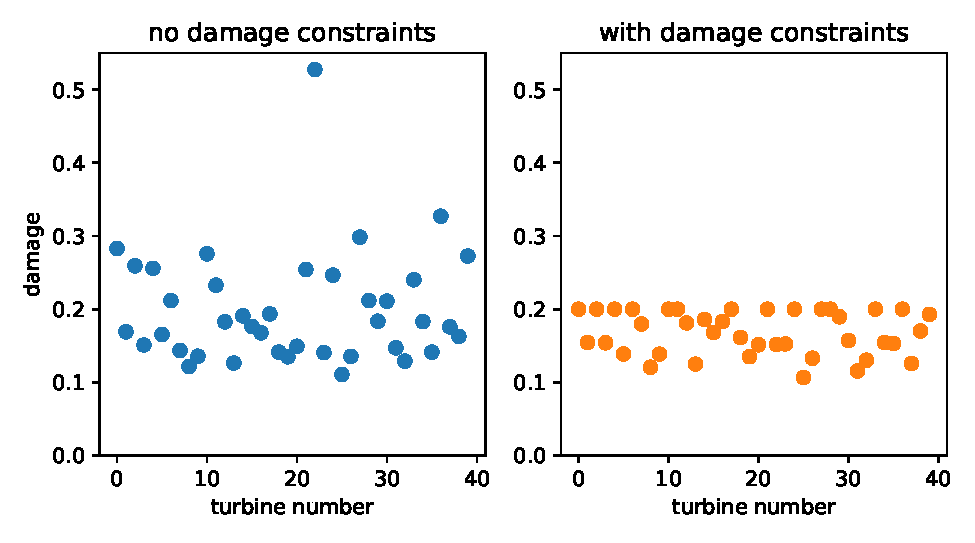
\includegraphics{images/opt_damage_vals.pdf}
    \caption{}
    \label{layouts}
\end{figure}

\section{Conclusions}

\section*{Code and data availability}


\section*{Author Contributions}


\section*{Competing Interests}
The authors declare no competing interests.



\bibliographystyle{unsrt}
\bibliography{references.bib}

\section*{Appendix 1: Large Eddy Simulation}
\label{sec:les}
\end{document}